\documentclass[11pt]{article}
\usepackage[margin=0.85in]{geometry}
\usepackage[T1]{fontenc}
\usepackage{lmodern,microtype,amsmath,amssymb,booktabs,graphicx,array,longtable,float}
\usepackage[numbers,sort&compress]{natbib}
\usepackage[hidelinks]{hyperref}
\usepackage[font=small,labelfont=bf]{caption}
\usepackage{enumitem}
\setlist{nosep,leftmargin=*}
\setlength{\emergencystretch}{2em}
\graphicspath{{../../artifacts/clarification_planning/figures/}}
\title{When Two Clarifications Are Worth More Than One:\\Budgeted Decision Planning for LLM Agent Work}
\author{OverseeingManyLLMs research draft\\\small Separate exploratory methods and results package}
\date{11 September 2026}
\begin{document}
\maketitle
\begin{abstract}
Several agents can depend on user decisions that are individually unhelpful but jointly sufficient to finish useful work. We formulate clarification as a budget-constrained decision protocol with explicit scope, uncertain interpretation, and terminal choices to release or defer deliverables. A bounded planner ranks unresolved dependencies in small completion blocks, evaluates contingent question sequences, executes one question, and replans. We compare it with one-step value of information, shared memory, full-history answering, and completion heuristics. A frozen evaluation uses 48 previously unused MultiWOZ dialogues and two GPU-generated interpretation replicates per dialogue. At a budget of two additional answers, two-step planning reduces dimensionless terminal loss relative to one-step selection by 0.240 per dialogue, with a paired 95\% interval of [0.115, 0.365] for the reduction. Its advantage over semantic memory is uncertain. More decisively, a secondary minimum-sufficient-completion audit achieves loss 62 versus the planner's 63 with 135 rather than 177 answers across 96 preparations. The dialogues support conjunctive requirements but no annotated sharing across deliverables. Synthetic tests establish a complementary-question mechanism and expose pruning and belief limitations. The study supports an executable decision protocol and a specific failure of myopic clarification. It does not establish a general advantage for the more elaborate planner, prevalence of shared scope decisions, or reduced human workload.
\end{abstract}

\section{The decision problem}
A user supervising several agents needs useful work to finish, rather than a large number of answered questions. A publishing agent might need an output format and an accessibility requirement before it can proceed. An implementation agent and a test author may depend on the same decisions. Answering an unrelated meeting question can complete one task immediately, whereas answering either publishing question alone may complete nothing. A one-question-at-a-time utility calculation can miss the joint opportunity.

This problem also has a strong alternative explanation. If completing a task is what matters, a simple policy could identify its missing requirements and ask for them. Moreover, the user may already have stated the answers. A capable full-history interpreter can then avoid clarification entirely. These alternatives make the empirical comparison more demanding than demonstrating a favorable lookahead example.

We investigate a protocol that connects task requirements, scoped decisions, and a pathwise response budget. Its implementation contribution is a bounded dependency-based candidate rule for contingent clarification planning, together with explicit stopping, release, and deferral semantics. Our empirical contribution is an auditable comparison that separates the mechanism from its practical value. We preserve the stronger simple comparator even though it weakens the algorithmic claim.

Earlier experiments in this repository found no retail search advantage, a mechanical no-review tie under the primary HVAC beliefs, harmful model review, and no overall attention-session advantage over sticky EDF. Those are historical evidence about different interventions. We neither reinterpret them as successes nor reuse their inspected cases as new evaluation data. The present question concerns acquiring user decisions, not ordering reviews of maintenance diagnoses.

\section{Relationship to established methods}
Value of information already balances communication benefit against its cost. Dong et al. formulate a clarify-or-commit decision with estimated intentions and response probabilities, and evaluate one-step hypothetical updates in their communication framework \citep{dong2026voi}. Our depth-one condition implements that decision rule with the same numeric beliefs and release objective as depth two. It is an adaptation of the rule, not a reproduction of their full LLM pipeline.

MAC coordinates ambiguity handling through a supervisor and domain agents \citep{acikgoz2026mac}. Its routing and one-question-per-turn procedure already establish that clarification can be coordinated across agents. Fleet auditing also models limited oversight, fallible confidence, and correlated errors \citep{zavattari2026fleet}. These works preclude a novelty claim for sharing oversight or asking centrally. Shared memory is another direct alternative. Our small-store memory comparator uses all source-checked records; it is not a reproduction of Mem0's full extraction, retrieval, and graph architecture \citep{chhikara2025mem0}.

The closest mathematical predecessor is preference elicitation as a partially observable Markov decision process. Boutilier explicitly motivates nonmyopic elicitation and models noisy responses, terminal actions, and Bellman values \citep{boutilier2002elicitation}. Krause and Guestrin study budgeted observation selection and conditional plans, exploiting graphical structure and characterizing computational limits \citep{krause2005nonmyopic}. Our task dependency representation specializes these established ideas. It does not introduce Bellman planning or a new general information-gathering objective.

Adaptive submodularity can justify greedy policies when information has diminishing returns \citep{golovin2011adaptive}. Conjunctive task completion need not satisfy that property. Our counterexample explains why one-step selection can fail, but supplies no submodular approximation guarantee. The strongest competing explanation for an observed gain remains a simple completion heuristic. Section~\ref{sec:audit} tests that explanation directly. The accompanying literature matrix identifies inspected sections and released-code limitations.

\section{A budgeted decision protocol}
\subsection{Public state and distinct deliverables}
Let $T$ be distinct user-valued deliverables and $D$ decision records. A record contains
\[
(\text{value},\text{scope},\text{exceptions},\text{source},\text{version},\text{status}).
\]
An inferred value is distinguished from a received user answer. A task $j$ registers required decisions $R_j$. Alternative bindings can use a shared decision when an applicability condition holds or a local answer when it does not. A value and the question of where that value applies are separate factors and separate substantive decisions. Repeating the same artifact under several agent names does not create additional utility.

The public state $s$ contains released text, declared task requirements, factor beliefs, represented scope conditions, received answers, versions, and attempted questions. The hidden state $\theta$ represents user intent, including applicability. The planner never receives unasked answers or evaluation labels. A task's multiple uses of a shared record refer to one factor. A shared mistake therefore affects all dependent tasks jointly, rather than being treated as independent corroboration.

\subsection{Loss and terminal actions}
Each task can be released using a valid binding or left unfinished. Define
\begin{equation}
L(a,\theta)=\sum_{j\in T}\left[e_j\mathbf{1}\{j\text{ released incorrectly}\}+d_j\mathbf{1}\{j\text{ unfinished}\}\right].
\end{equation}
Correct release has zero loss. We study
\begin{equation}
\min_\pi\;\mathbb{E}\left[L(a_{\rm final},\theta)+\lambda\sum_t c(q_t)\right]
\quad\text{subject to}\quad\sum_t c(q_t)\leq B\text{ on every path}.
\end{equation}
Primary weights are $e_j=4$, $d_j=1$, and $\lambda=0.05$. One atomic answer costs $c(q)=1$. These are dimensionless research assumptions. They are not money, time, or measured cognitive effort. Reported terminal loss excludes the separately reported question penalty. Sensitivities use $e_j=2$ and $8$.

For each binding, the terminal rule chooses the most probable releasable value for each required factor. It computes the binding's correctness probability under the estimated factor model and compares $e_j(1-p_j)$ with $d_j$. Equality defers. A binding cannot consume an explicitly excepted or non-allowed record. No terminal action consults the evaluator's answer. These controls are identical across the mechanism comparisons.

\subsection{Beliefs and responses}
The implementation stores finite categorical factors for values and separate Boolean factors for applicability. Distinct factors are assumed independent. Shared references remain one factor. Independence is an approximation for natural-language interpretation and is deliberately violated in a sensitivity condition.

A supplied empirical value receives a development-fitted probability of correctness. The remaining probability is assigned to an unspecified alternative, OTHER. Missing values have all probability on OTHER. Before a response, OTHER is not a releasable answer. A question can reveal a concrete value from that category. This representation does not look up the correct value to populate the hypothesis space.

The primary response channel returns an accurate source-label answer to an actually asked question. This is a simulated user with sufficient knowledge, not another model or a human participant. Synthetic conditions separately add symmetric categorical response error of 0.2 or unresolved-response probability of 0.3. Updates use the declared likelihood and Bayes' rule. An unresolved answer consumes budget, conveys no information, and cannot be requested again during the same version. Registered revisions are public events and never reset spent budget.

\subsection{Finite-horizon planning}
With remaining budget $b$, define
\begin{align}
V_0(s,b)&=\min_a\mathbb{E}[L(a,\theta)\mid s],\\
V_h(s,b)&=\min\left\{V_0(s,b),\;\min_{q:c(q)\leq b}\left[\lambda c(q)+\sum_y P(y\mid s,q)V_{h-1}(U(s,q,y),b-c(q))\right]\right\}.
\end{align}
$U$ records the received answer, updates its posterior, and marks the question attempted. Responses are predicted from public beliefs and the declared channel. The controller executes only the first question of the selected contingent plan, receives its actual response, and replans. It can stop with some tasks released and others deferred. There are no added deadlines or simulated human response durations in this experiment.

\section{Bounded dependency planning and properties}
The approximate algorithm constructs completion blocks containing up to three unresolved factors from a task binding. It ranks each block by an optimistic reduction in task loss per answer, setting block factors to certain while retaining the other beliefs. Each factor receives the larger of its best block score and immediate value of information. This keeps some zero-immediate-value complementary questions in consideration. The subsequent contingent recursion evaluates expected value; the optimistic ranking is not credited as achieved benefit.

At each node, at most eight factors are expanded. When eight or fewer are available, every question is included. Depths one and two are core conditions; depth three is a sensitivity. A 25,000-state expansion limit substitutes terminal loss at unexplored nodes and records the cap. Belief states, attempted/revealed masks, budget, and depth support memoization. Changed alphabets or revisions rebuild the relevant planner. A generic-search ablation uses the same width and depth but ranks questions by immediate value alone.

\paragraph{Budget adherence.} Initially expenditure is zero. Proposal and response handlers both reject unaffordable questions. A resolved or unresolved response adds its positive cost exactly once. Induction over events gives expenditure at most $B$ after every response, independently of which response branch occurs. Revisions do not create additional budget. Unsolicited user updates are logged separately from solicited clarifications.

\paragraph{Represented scope and versions.} Every release registers the versions of its consumed value and applicability records. A changed dependency invalidates that release, while unrelated records retain their versions. The release guard rejects a mismatch. The online implementation, SafeProtocol, increments versions for both explicit revisions and newly resolved answers following an earlier release. It also checks explicit exceptions on applicability records. This invariant assumes complete registered dependencies and use of the guard. It does not prove semantic applicability or discover an omitted dependency. A version-update defect in the initial interactive implementation was repaired separately; terminal-only experimental outcomes are unaffected.

\paragraph{Complementarity counterexample.} Let two independent uniform binary answers $q_1,q_2$ jointly determine three distinct deliverables. A third answer $q_3$ determines a fourth. At $e=4,d=1$, a task with any unknown binary requirement defers. Clarifying $q_1$ alone saves zero, but clarifying it after $q_2$ saves three. Marginal benefit increases, violating diminishing returns. With two available answers, one-step selection chooses $q_3$ and stops at loss three. Two-step planning chooses $q_1,q_2$ and ends at loss one. This authored example demonstrates a mechanism, not its prevalence.

\paragraph{Depth-one equivalence and complexity.} Setting $h=1$ compares $V_0$ with the question penalty plus expected post-question terminal loss. This is exactly the implemented one-step baseline with identical candidates and ties. If at most $k+1$ response branches and $w$ questions are expanded, a loose recursion bound is $O((w(k+1))^h C)$ for terminal cost $C$. Completion-block construction additionally enumerates subsets of size at most three within each binding. The independent exact reference expands every question for at most six factors and budget six. Pruning can lose the best sequence, and no general optimality guarantee is claimed.

\begin{figure}[t]
\centering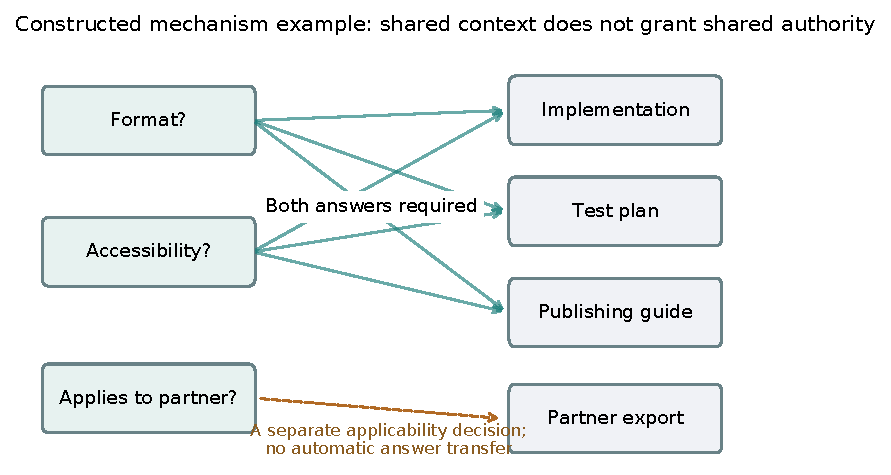
\includegraphics[width=.94\linewidth]{dependency_example.pdf}
\caption{Authored mechanism example. Registered value dependencies can be shared; an exceptional task needs its own value or a separate applicability decision. The graph is constructed, not extracted evidence of real shared authority. Question cost counts values and scope separately.}
\end{figure}

\section{Experimental design}
\subsection{Frozen source-grounded comparison}
The source is MultiWOZ 2.4 \citep{ye-etal-2022-multiwoz}, pinned to revision \texttt{6807c1d}. Human-authored task dialogues supply utterances; benchmark records supply databases and annotated current constraints. Agent roles and deliverables are our adaptation. We select one executable shortlist per supported domain, using hotel, restaurant, and attraction fields. A shortlist succeeds only when its normalized required constraints match the annotation and execution returns the corresponding records. An empty correctly constrained query is a completed artifact, not a completed booking.

We release the complete source dialogue. We do not mask known answers to manufacture complementarity. Supported field names define the public task interface; their annotated values and lexical-support metadata remain evaluator-only. This oracle-provided task schema is a limitation of the adaptation. The model must still interpret actual values and source references from text.

Selection takes the first eligible lexicographic IDs from the official validation and test splits, requiring at least two supported domains and at most 4,500 source characters. We exclude all 33 historically used or inspected dialogues, exact dialogue duplicates of them, and repeated selected goal signatures. The initial development screen admitted single-domain cases and was revised before evaluation. All 18 newly exposed development dialogues are retained in the audit; twelve final development dialogues fit probabilities. The 48 fresh evaluation dialogues have no ID or exact selected-goal overlap with development. Public-benchmark pretraining contamination remains unknown.

Each dialogue has two generation replicates. We make three serial GPU calls per preparation: source-linked record extraction, answering from all current source-checked memories, and full-history answering. Qwen2.5-7B-Instruct uses revision \texttt{a09a3545}, BF16 on one RTX 6000 Ada, temperature 0.3, top-$p$ 1, and no CPU offloading. Maximum context is 2,048 tokens; output limits are 640 tokens for extraction and 256 otherwise. All actual requests fit. Seeds do not imply bitwise reproducibility. Controlled planning methods reuse each saved memory interpretation and the same accurate simulated answers. Full history is a distinct interpretation comparison, with fewer upstream generation steps, rather than a pure planning ablation.

The probability that a supplied value is correct is estimated by Beta(1,1) smoothing per backend/domain, falling back to its backend's pooled estimate below ten examples. The fitted development set contains no attraction cases, so that domain uses the declared fallback. Missing values are unknown rather than confident guesses. The estimator is frozen before evaluation and never updated from evaluation labels.

The freeze commit \texttt{397c7a32} precedes held-out generation. It contains source IDs, prompts, model settings, beliefs, synthetic configurations, policy definitions, error weights, and analysis code. Budgets are 0, 1, 2, 4, 6, and enough to ask all represented unresolved factors. The two primary contrasts are depth two minus one-step and depth two minus semantic memory at budget two and $e=4$. The unit is a source dialogue. We average its two replicates and resample all matched conditions together, using 2,000 paired bootstrap resamples and seed 82164. Intervals are descriptive marginal intervals, with no multiplicity correction. Replays and agent roles are not additional independent samples.

\subsection{Comparators and synthetic design}
All common methods share terminal release rules, question costs, scope controls, and user responses. Semantic memory asks missing fields in task order. Full history uses the same clarification wrapper with its separately calibrated interpretations. One-step VoI equals depth one. The declared completion heuristic picks the task with the fewest still-queryable factors, ties by current loss per question cost, and asks its least certain factor. Depth three, generic search, disabled scope questions, request-specific records, and ideal annotation interpretation are diagnostic conditions. Budget zero supplies a no-question control. The stronger completion audit in Section~\ref{sec:audit} is explicitly secondary.

Synthetic development and evaluation seeds are disjoint. Fourteen named families cover independent, shared, complementary and mixed tasks, scope and exceptions, wrong sharing, revision and revocation, imperfect or unresolved responses, already sufficient memory, zero value, distractor pruning, and misspecified beliefs. Twenty evaluation seeds per family yield 280 instances. Nine overlap/requirement-arity configurations use twelve additional seeds each, yielding 108 more. These are 388 configuration/seed instances, not 388 independently authored source problems. Seeds repeat across configurations. Ten methods and six budgets produce 23,280 saved replay rows.

An audit found inconsistent direct local answers in two scope families. Thirteen of their 40 instances could answer a local question inconsistently with the effective target. We preserve those invalid original rows and rerun the same 40 cases with that answer corrected in a separate 2,400-row artifact. Reported valid synthetic summaries combine 348 unaffected instances with 40 explicitly post-freeze corrected sensitivities. The repair creates correlations that the factorized planner does not model exactly. No GPU generation or empirical outcome is altered.

\section{Results}
\subsection{Primary outcomes and their components}
Table~\ref{tab:primary} reports totals across 96 preparations and 192 distinct task preparations. The statistical sample remains 48 dialogues. Depth two saves 23 terminal loss points relative to one-step selection, corresponding to a mean paired difference of $-0.2396$ per dialogue, 95\% interval $[-0.3646,-0.1146]$. It wins on 17 dialogues, ties on 29, and loses on two. It completes 23 more deliverables correctly with the same two incorrect releases, but asks 45 additional questions.

Relative to semantic memory, depth two's difference is $-0.0938$ with interval $[-0.2188,0.0104]$, and six wins, 40 ties, and two losses. This does not establish a reliable loss advantage. Whole-project completion also differs from per-task quality: the planner completes 39 projects across replicates, versus memory's 41 and full history's 45. A gain in weighted loss must not be described as a universal gain in user goals.

\begin{table}[t]
\centering\small
\caption{Budget two, error weight four. Totals over 96 preparations, with 192 task preparations. Questions are additional simulated user answers. Whole means both domain tasks correct. The starred audit is secondary.}
\label{tab:primary}
\begin{tabular}{lrrrrrrr}\toprule
Method & Loss & Correct & Wrong & Unfinished & Whole & Questions\\\midrule
Semantic memory &72&129&3&60&41&160\\
Full history &82&140&10&42&45&3\\
One-step VoI &86&112&2&78&37&132\\
Fewest queryable answers &77&118&1&73&22&192\\
Two-step planner &63&135&2&55&39&177\\
Minimum sufficient completion* &62&139&3&50&44&135\\
Ideal interpretation &0&192&0&0&96&0\\\bottomrule
\end{tabular}
\end{table}

\begin{figure}[t]
\centering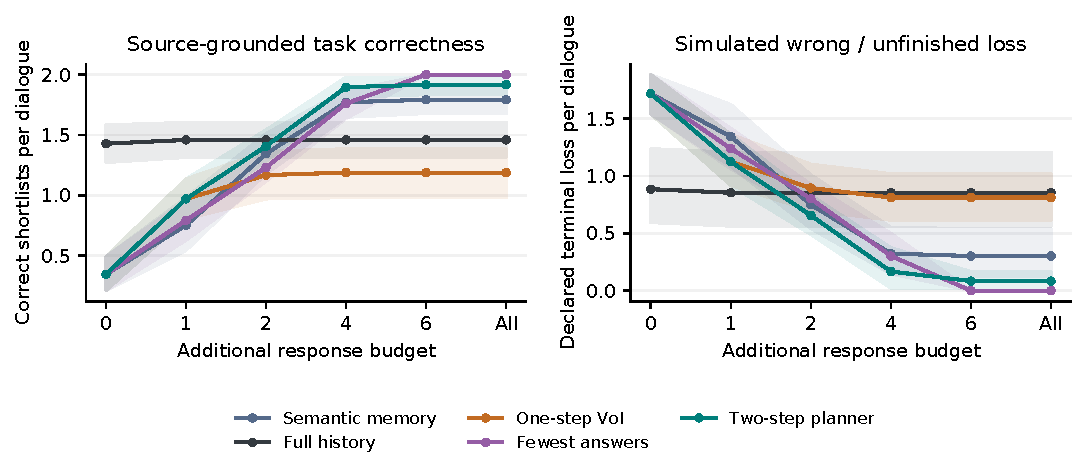
\includegraphics[width=\linewidth]{empirical_quality_budget.pdf}
\caption{Source-grounded task outcomes under simulated extra responses and loss weights. Shading is a 95\% bootstrap interval over 48 dialogue means. The identical memory preparations support the planner, one-step, and completion comparisons. Full history uses its own saved interpretation. ``All'' allows every represented question; it does not force asking.}
\label{fig:budget}
\end{figure}

\subsection{A stronger simple explanation}\label{sec:audit}
The declared completion heuristic counts every still-queryable factor, even when fewer answers would suffice to cross the common release threshold. Before inspecting completed primary summary tables, we documented a secondary comparator audit to address this concrete weakness. Minimum sufficient completion enumerates the cheapest affordable dependency subsets that make a currently deferred task releasable under every supported response path. It ties by expected task loss saved per question cost, then stable IDs. It asks one question and reconsiders. It sees no labels and uses no additional generations. This audit is not a new confirmatory sample.

The simpler rule obtains loss 62 versus the planner's 63, with 135 rather than 177 questions. The planner-minus-audit loss difference is $+0.0104$, interval $[-0.1146,0.1042]$, with one win, 44 ties, and three losses. The planner asks an additional 0.4375 answers per dialogue, interval $[0.3021,0.5729]$. The audit also completes four more tasks correctly and five more whole projects, while making one additional incorrect release. These point estimates favor simplifying the practical controller. A wide interval does not prove equivalence, but the data do not support claiming that the more elaborate algorithm improves this application overall.

\begin{figure}[t]
\centering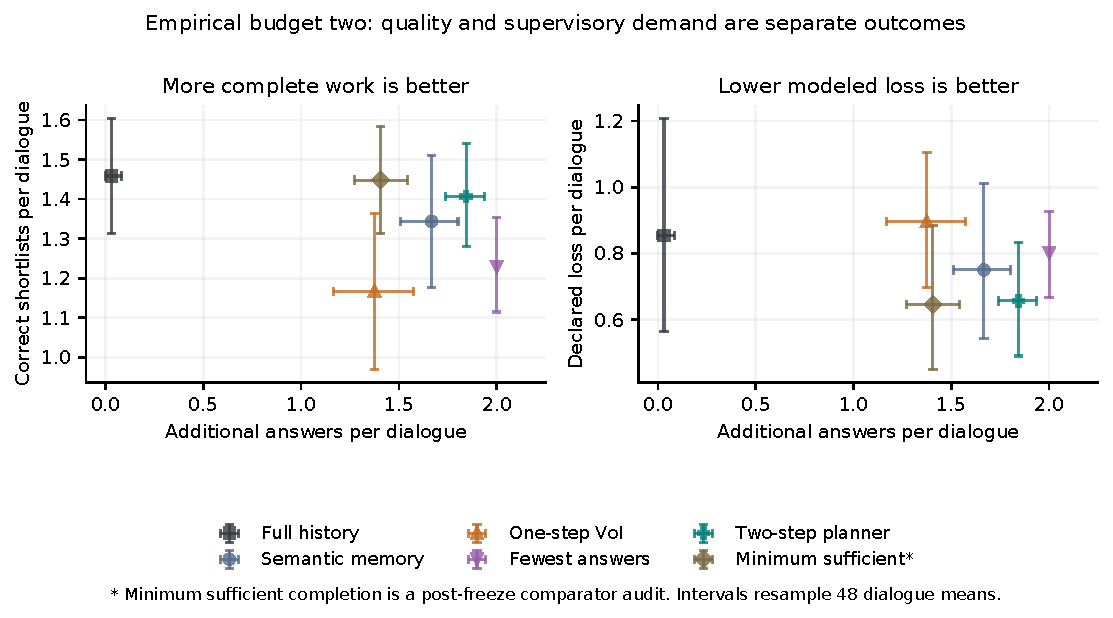
\includegraphics[width=\linewidth]{quality_effort_audit.pdf}
\caption{Quality and modeled supervisory demand at budget two. Horizontal and vertical intervals resample the same source dialogue units. The starred completion comparator is a post-freeze audit using unchanged preparations. All answers and downstream releases are simulated; no cognitive-load measurement is implied. Its point estimate offers nearly the planner's loss with fewer questions.}
\end{figure}

\subsection{What the dialogues actually test}
There are 96 source-derived shortlists with 191 constraints. Seventy-three tasks require at least two fields. In the generated memory condition, 70 of 192 task preparations are missing at least two values. Depth one and two choose different first actions in 47 of 96 preparations, spanning 25 dialogues. In 21 preparations spanning 13 dialogues, depth one stops while depth two asks. This supports the claimed myopic-stopping mechanism on imperfect interpretations.

However, all required values were already present in source text. Source-checked extraction supplies only 148 of 382 evaluation field preparations, and memory answering supplies 160. Full history supplies 379. Conditional on supplying a value, correctness is 147/148 for extraction, 152/160 for memory, and 363/379 for full history. A total of 143 extracted records fail the public source guard. Asking the user often repairs an extraction or provenance bottleneck rather than obtaining genuinely absent intent.

No annotation establishes a shared decision across domain deliverables. The empirical adapter therefore has zero shared factors across tasks. Request-specific and disabled-scope ablations are identical to the planner here for structural reasons. Depth three cannot exceed depth two at budget two. Generic depth-two search also ties because all empirical candidate sets fit within width eight. These ties provide no evidence for the distinctive candidate construction or scope-acquisition feature. Memory interpretations differ between generation replicates on 21 fields across 14 dialogues. Planner losses differ in three dialogues, whereas one-step losses differ in eleven. These are different-seed preparations, not a repeated-identical-request test.

Full history's 3 questions versus the planner's 177 are a substantial practical contrast. At primary weights, its additional wrong releases produce higher loss, with an uncertain paired difference. At error weight two, full history is better: planner minus history is $+0.2604$, interval $[0.0417,0.4688]$. At error weight eight, the difference reverses to $-0.8333$, interval $[-1.1250,-0.5417]$. Thus a preference for fewer questions or a different tolerance for incorrect release changes the conclusion. Ideal interpretation completes every task with zero questions. This confirms that clarification is not intrinsically necessary for these complete source conversations.

\subsection{Synthetic mechanism, approximation, and fallibility}
The transparent complementary fixture realizes loss one for depth two and loss three for one-step or the declared completion rule at budget two. Independent-question and already-sufficient-memory conditions include ties. At budget four with three jointly required answers and full task overlap, depth two has three more loss points than the simple completion heuristic. Its short horizon cannot see the full three-answer payoff, whereas the heuristic commits to finishing the task. This is a structural counterexample to a broad lookahead advantage, not a rare model failure. The overlap/arity map in the appendix shows where the imposed task structure creates gains and where it does not. Such designed examples establish capability, not practical frequency.

The frozen small-instance suite yields 220 depth-two comparisons at each of widths two and eight with no positive approximation gap beyond floating-point tolerance. This finite check is not a guarantee. A separate authored six-factor pruning witness has a gap of 1.2 at width two: individually larger standalone candidates exclude both roots of a complementary pair. It explicitly demonstrates how the ranking can fail. The twelve-factor distractor family shows why dependency blocks can help against generic bounded search, but that structure has no empirical counterpart here.

Corrected scope families and imperfect-response conditions remain visible even when they yield no advantage. A local clarification alternative can make a scope question unnecessary. Simulated accuracy and belief factorization govern the achievable gain. The protocol's version and scope invariants cannot protect against a semantically wrong belief or an incomplete registered dependency.

Mean measured CPU episode time is 1.34 ms for empirical depth two, 0.65 ms for one step, and 0.55 ms for the declared completion heuristic. Synthetic depth two averages 6.71 ms and depth three 27.89 ms. No evaluated primary or synthetic selection reaches the state cap. These measurements describe small instances on this host, not general fleet scaling.

\section{Prototype, reproducibility, and limitations}
The local Decision desk charges a changed scope separately from the value answer, even when they appear on one card. It exposes selectable planners, a proposed question, its scope, potentially enabled work, whether another answer may be needed, and the remaining budget. It preserves narrowly answered exceptions, unresolved work, manual overrides, revisions, and revocations. Expandable provenance keeps algorithm details outside the main decision flow. A public Python adapter and localhost API support the demonstration. Fifteen browser checks record displayed questions, actions, intervals, and state hashes. These are scripted software interactions, not participant observations.

The package preserves every model attempt and deterministic replay trace. It uses 396 calls and 396 attempts, including all 108 development calls and 288 held-out calls, with zero retries or transport/parse failures. Usage is 174,262 prompt and 25,545 completion tokens. Summed generation latency is 604.67 seconds; it is not billed allocation time. CUDA BF16 execution and unchanged zero-offload server arguments are saved. All policy comparisons and audits require zero further generations. Resource clocks are separately recorded and the original 36-hour history remains unchanged.

The strongest limitations concern what the experiment represents. The additional user is perfect in the primary study. Required field names are provided by the adapter. Source text is short and complete. Calibration has only twelve development dialogues and no attraction examples. The finite belief representation cannot describe arbitrary response meanings, and independently modeled factor errors can be correlated. Database templates and unknown shared source participants limit independence claims. No human reading time, experienced workload, or decision quality was observed. Source annotations are not real-world preference verification. These limits motivate a narrower contribution rather than a general superiority claim.

\section{Conclusion}
Budgeted clarification can have complementary value, and a one-step policy can stop when two answers would complete useful work. We provide an executable protocol, a bounded dependency planner, and a paired evaluation that isolates this behavior. The empirical advantage does not survive as a broad practical claim against a stronger completion heuristic. Full-history interpretation also avoids most extra questions, and the dialogue adaptation does not establish legitimate cross-task sharing. The supported next step is to use minimum sufficient completion as the practical default and collect tasks with independently justified shared decisions before expanding the planner. The formal mechanism is worth retaining; a general algorithmic advance remains unproven.

\appendix
\section{Additional paired and diagnostic evidence}
All plots are generated from saved numerical tables. Teal negative paired differences favor depth two; unfavorable regions remain visible. Figure selection uses the first lexicographic source dialogue with a negative, zero, or positive replicate-averaged loss difference, never the largest effect. Both replicates of each selected dialogue are displayed. This expands the original replicate-zero display without changing the frozen selection of dialogues.

\begin{figure}[H]
\centering
\includegraphics[width=\linewidth]{paired_differences.pdf}
\caption{Empirical per-dialogue paired differences at budget two and error weight four. Source dialogues are the units; each bar averages two generated interpretations. Policy outcomes use simulated responses and declared losses. Negative means lower loss for two-step planning.}
\end{figure}
\begin{figure}[H]
\centering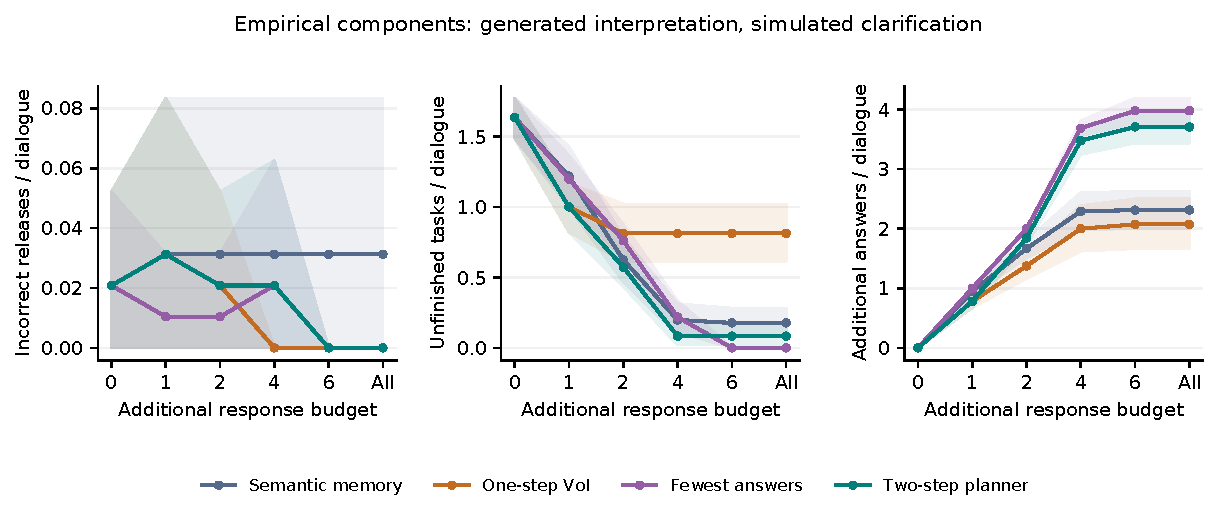
\includegraphics[width=.9\linewidth]{empirical_components.pdf}
\caption{Empirical wrong and unfinished releases under simulated response budgets. These components remain separate from total loss. The task labels come from benchmark annotations and executable shortlist checks, not a human study.}
\end{figure}
\begin{table}[H]
\centering\small
\caption{Secondary generation and coverage diagnostics. Coverage counts field preparations, while variation counts source dialogues out of 48. Different generation seeds and, for memory, possibly different extracted inputs are involved.}
\begin{tabular}{lrrr}\toprule
Backend & Supplied / 382 & Correct when supplied & Dialogues differing by replicate\\\midrule
Source-checked extraction &148&147&13\\
Memory answering &160&152&14\\
Full-history answering &379&363&4\\\bottomrule
\end{tabular}
\end{table}
The source-guard coverage bottleneck is distinct from a transport failure. Every
call completed and parsed, but a record can still be rejected or an answer can be
missing or incorrect. These cases remain in the release and deferral outcomes.
The values were already stated by source users, so additional questions here
repair interpretation gaps rather than establish the prevalence of missing intent.

\clearpage
\begin{figure}[H]
\centering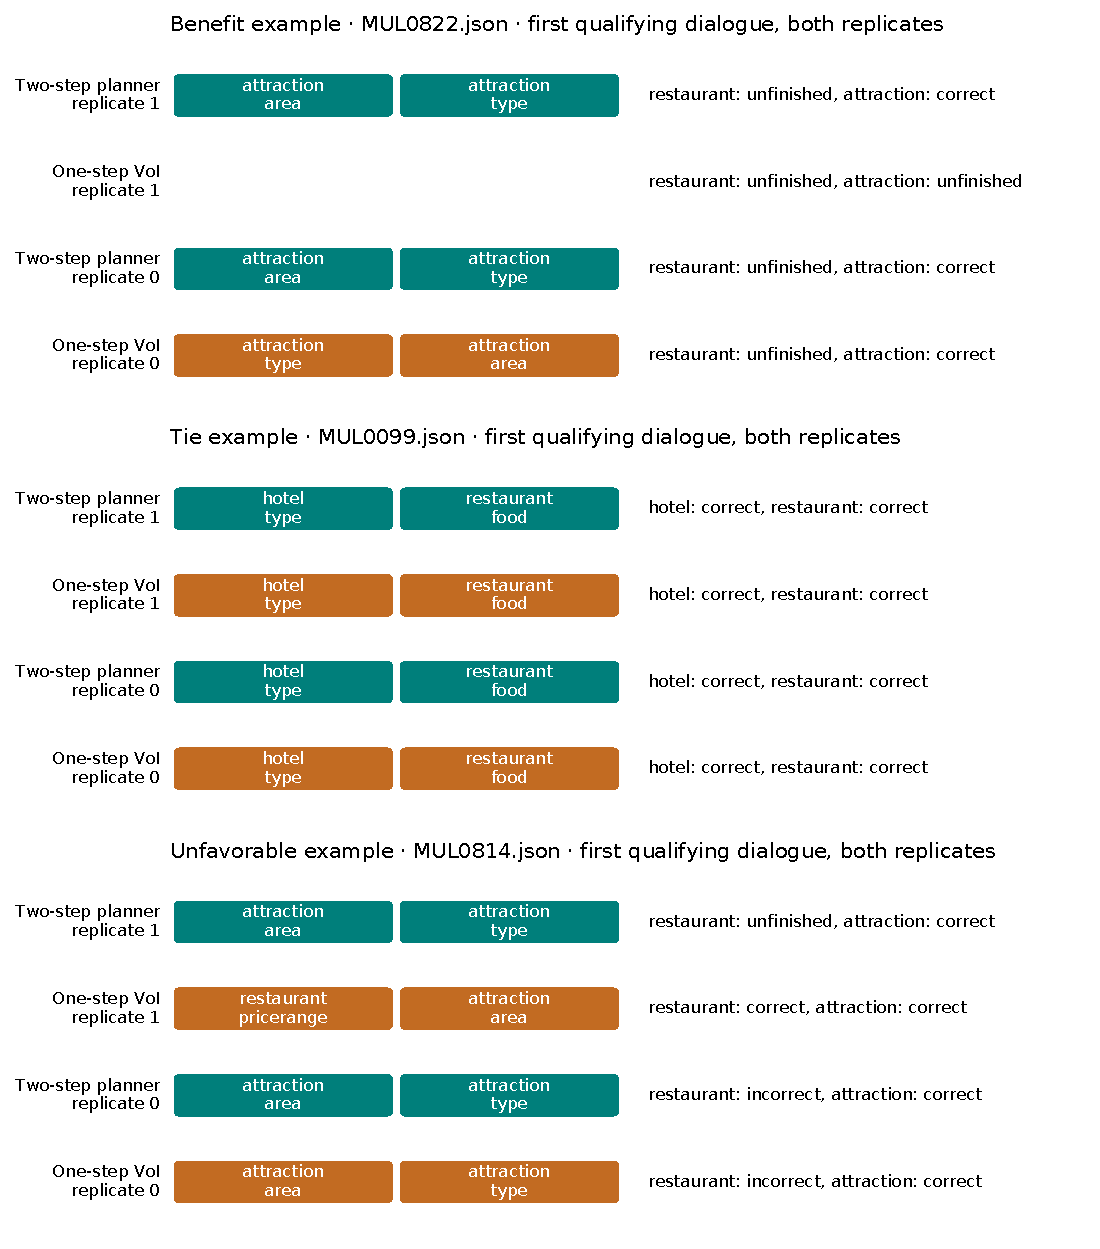
\includegraphics[width=.98\linewidth,height=.85\textheight,keepaspectratio]{matched_questions.pdf}
\caption{First qualifying favorable, tied, and unfavorable dialogues by the declared rule. Both generation replicates appear. Blocks are actual displayed atomic questions in saved policy replays, with source-derived constraints and simulated answers. Horizontal position is question order, not measured response time.}
\end{figure}
\clearpage
\begin{figure}[H]
\centering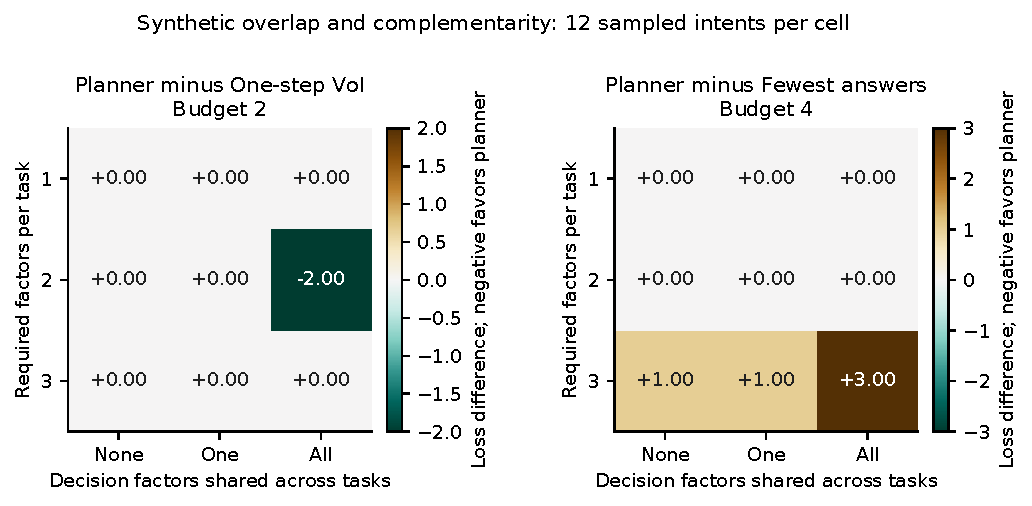
\includegraphics[width=\linewidth]{synthetic_overlap_map.pdf}
\caption{Fully synthetic dependency sensitivity. The left panel compares one-step at budget two; the right compares fewest answers at budget four and retains a region where the planner is worse. Overlap and arity are authored, and all values, answers, and losses are simulated. The plot tests the designed structural mechanism; it does not estimate the prevalence of such tasks in human work.}
\end{figure}
\begin{figure}[H]
\centering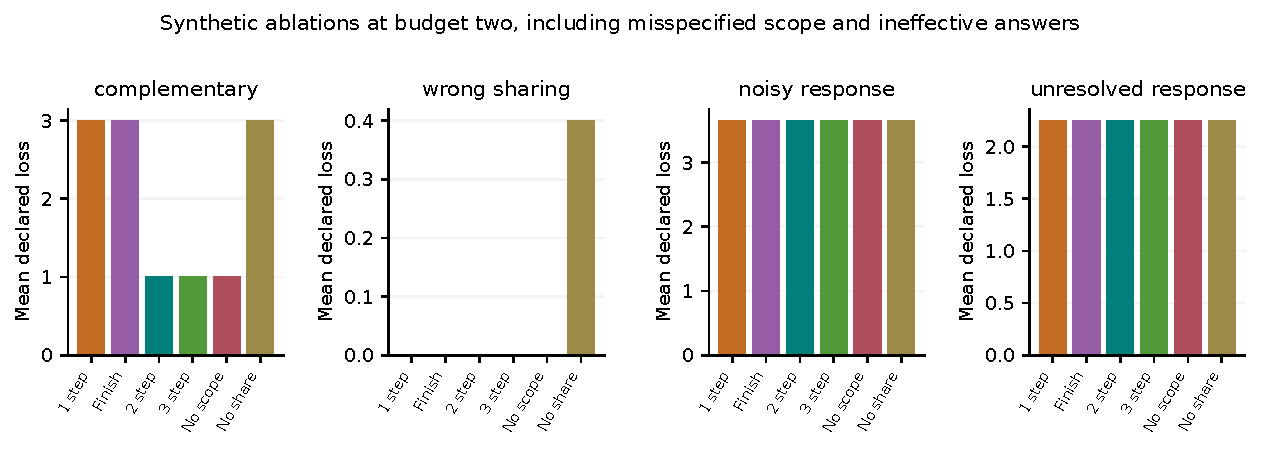
\includegraphics[width=\linewidth]{synthetic_ablations.pdf}
\caption{Synthetic mechanism ablations. The valid summaries preserve unaffected frozen rows and use separately repaired scope-response sensitivities for the two inconsistent families. Scope acquisition can tie because a local value question is an alternative. No human behavior is measured.}
\end{figure}
\clearpage
\begin{figure}[H]
\centering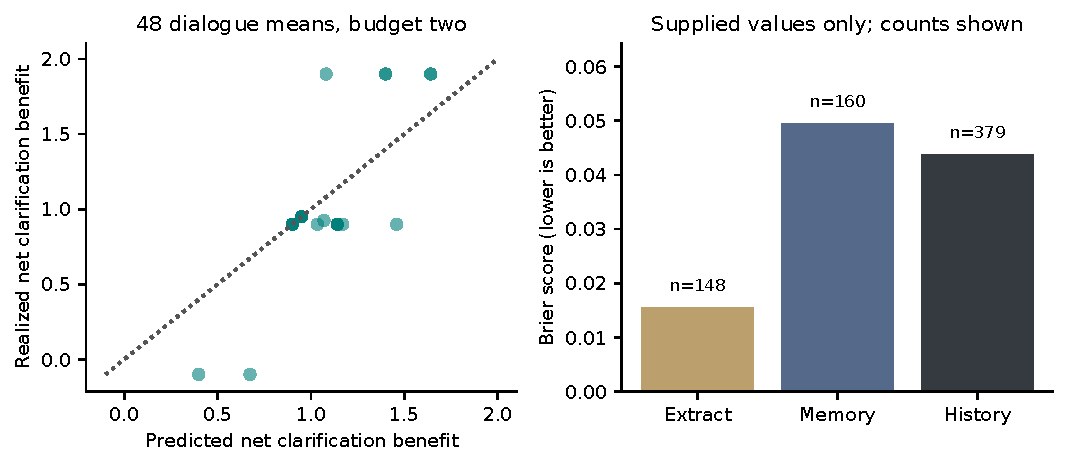
\includegraphics[width=\linewidth]{belief_diagnostics.pdf}
\caption{Left: estimated two-step net benefit before any answer versus realized benefit after simulated answers, including the question penalty. Right: conditional prediction reliability among supplied GPU-interpreted fields against source annotations, with counts. Missing-field coverage is reported in the text. Prediction error is retained.}
\end{figure}
\begin{figure}[H]
\centering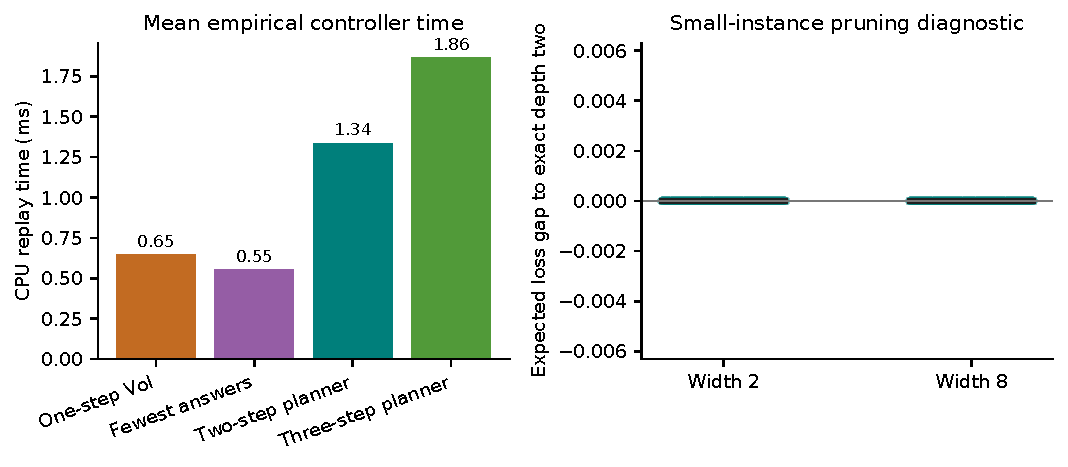
\includegraphics[width=\linewidth]{planning_cost_gap.pdf}
\caption{Measured host computation and exact-reference comparisons on authored small instances. Latencies are orchestration measurements, not human review time. Zero gaps in this finite suite do not establish optimality; the separate width-two witness has a gap of 1.2.}
\end{figure}
\clearpage
\section{Inspectable interaction and reproduction}
\begin{figure}[H]
\centering
\includegraphics[width=\linewidth]{../../artifacts/clarification_planning/interface/planned_question.png}
\caption{Working local interface with an authored five-deliverable example. It explains shared requirements, scoped alternatives, and deferred work. This screenshot and its saved interactions are a scripted demonstration, not participant data.}
\end{figure}

From the repository root, saved-output verification is
\begin{verbatim}
python3 -m research.clarification_planning.reproduce \
  --figures --output /tmp/clarification-reproduction
python3 research/clarification_planning/prototype/server.py
bash paper/clarification_planning/build.sh
\end{verbatim}
The README documents focused tests, source archive verification, fresh-generation limitations, and the adapter. Frozen code and declarations remain immutable; separate files document the stronger comparator, synthetic responder repair, and online version fix. The historical submission sources are unchanged. Figure data, raw requests, traces, and manifests are under \texttt{artifacts/clarification\_planning/}.

\clearpage
\bibliographystyle{plainnat}
\bibliography{references}
\end{document}
